% Dit werk is gelicenseerd onder de licentie Creative Commons Naamsvermelding-GelijkDelen 4.0 Internationaal. Ga naar http://creativecommons.org/licenses/by-sa/4.0/ om een kopie van de licentie te kunnen lezen.
\documentclass[t]{beamer}

\usepackage{xcolor}						% Om kleuren te gebruiken
\usepackage[dutch]{babel}               % Voor nederlandstalige hyphenatie (woordsplitsing)
\usepackage{amsmath,amsthm}             % Uitgebreide wiskundige mogelijkheden
\usepackage{url}                        % Om url's te verwerken
\usepackage{graphicx,subfigure}         % Om figuren te kunnen verwerken
\usepackage[utf8]{inputenc}             % Om niet ascii karakters rechtstreeks te kunnen typen
\usepackage{multicol}
\usepackage{listings}					% Code weergeven
\usepackage{courier}					% Code lettertype
\usepackage{textcomp}
\usepackage[absolute,overlay]{textpos}

\lstset{language=Python,
        basicstyle=\footnotesize\ttfamily,
        tabsize=4,
        breaklines=true,
        showstringspaces=false,
        upquote=true,
        xleftmargin=0cm,
        xrightmargin=0cm,
        backgroundcolor=\color{black!5!white}}
        
%%%%%%%%%%%%%%%%%%%%%%%%%%%%%%
% Layout
%%%%%%%%%%%%%%%%%%%%%%%%%%%%%%
\usetheme{Frankfurt}
\usefonttheme[onlymath]{serif}
\AtBeginSection[]
{
  \begin{frame}
    \frametitle{Inhoud}
    \tableofcontents[currentsection]
  \end{frame}
}

\setbeamertemplate{navigation symbols}{}
\setbeamertemplate{footline}[page number]

%%%%%%%%%%%%%%%%%%%%%%%%%%%%%%
% Title
%%%%%%%%%%%%%%%%%%%%%%%%%%%%%%
\title{Inleiding tot Python}
\author{Brecht Baeten\inst{1}}
\institute{
	\inst{1}%
  		KU Leuven, Technologie campus Diepenbeek,\\ e-mail: brecht.baeten@kuleuven.be
}
\date{\today}

\subtitle{}


\begin{document}
\frame{\titlepage}
\begin{frame}
	\frametitle{Wat is Python?}
	\begin{textblock}{6}(8,3)
            
\includegraphics[width=6cm]{fig/pythonlogo}
        \end{textblock}
	
	\vspace{2cm}
	
	\begin{itemize}
		\item Programeertaal
		\item Zeer object georienteerd
		\item Packages voor wetenschappelijke toepassingen
		\item Gratis
		\item Verschillende GUI's beschikbaar, niet meegeleverd
		\item Zéér verscheiden toepassingsgebied (Wetenschappelijke berekeningen, Web toepassingen, GUIs, quick scripting)
	\end{itemize}
\end{frame}
%%%%%%%%%%%%%%%%%%%%%%%%%%%%%%%%%%%%%%%%%%%%%%%%%%%%%%%%%%%%%%%%%%%%%%%%%%%%%%%%%
\begin{frame}
	\frametitle{Installatie}
		
	\begin{onlyenv}<1>
		\textbf{Mac}
		\begin{itemize}
			\item 2.7 standaard meegeleverd bij Mac OS X
		\end{itemize}
		
		\textbf{Linux}
		\begin{itemize}
			\item 2.7 standaard meegeleverd bij veel distributies
		\end{itemize}
		
	\end{onlyenv}
	\begin{onlyenv}<2>
		\textbf{Windows}
		\begin{itemize}
			\item Download een distributie (best 2.7 of 3.5) via \url{https://www.python.org/downloads/}
			\item Voeg Python toe aan het windows pad
			\item Download een degelijke text editor, bv. Notepad ++ \url{https://notepad-plus-plus.org/download/}
			\item Download een degelijke console, vb. ConEmu \url{http://sourceforge.net/projects/conemu/files/latest/download}
		\end{itemize}
		of
		\begin{itemize}
			\item Anaconda \url{https://www.continuum.io/downloads}
			\item WinPython \url{https://winpython.github.io/}
			\item Python(x,y) \url{http://python-xy.github.io/}
		\end{itemize}
	\end{onlyenv}
\end{frame}
%%%%%%%%%%%%%%%%%%%%%%%%%%%%%%%%%%%%%%%%%%%%%%%%%%%%%%%%%%%%%%%%%%%%%%%%%%%%%%%%%
\begin{frame}[fragile]
	\frametitle{Interactieve console}
    \begin{textblock}{6}(8,4)
        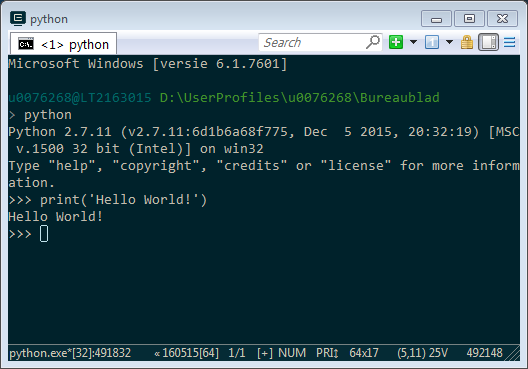
\includegraphics[width=6cm]{fig/commandwindow}
    \end{textblock}
    	
    \begin{itemize}
    	\item Open een console en typ "\lstinline{python}"
		\item Commando's uitvoeren
		\item variabelen definieren
		\item functies aanroepen
		\item Goed voor korte tests
		\item Sluiten met \lstinline[language=bash]{Ctrl + Z}
	\end{itemize}
	
    \vspace{2cm}
    
	\begin{lstlisting}
>>> print('Hello World!')
>>> x = 5
>>> x
>>> y = 4*x+x**2
>>> y
	\end{lstlisting}
\end{frame}
%%%%%%%%%%%%%%%%%%%%%%%%%%%%%%%%%%%%%%%%%%%%%%%%%%%%%%%%%%%%%%%%%%%%%%%%%%%%%%%%%
\begin{frame}[fragile]
	\frametitle{Scripts}
	\begin{textblock}{6}(8,3)
        %\includegraphics[width=6cm]{fig/available}
    \end{textblock}
    
	\begin{itemize}
		\item Opeenvolgende commando's opgeslagen in een .py bestand
		\item Aanroepen vanuit het command prompt
		\item Bestanden in de map waarin je python start zijn beschikbaar
		\item Met "\lstinline[language=bash]{-i}"\ als argument start een ineractieve sessie na het uitvoeren van het script 
	\end{itemize}
	
	\vspace{1cm}
	
	\begin{lstlisting}[language=bash]
> python -i hello_world.py
	\end{lstlisting}
\end{frame}
%%%%%%%%%%%%%%%%%%%%%%%%%%%%%%%%%%%%%%%%%%%%%%%%%%%%%%%%%%%%%%%%%%%%%%%%%%%%%%%%%
\begin{frame}[fragile]
	\frametitle{Variabelen}

	\begin{itemize}
		\item Int
		\item Float
		\item List
		\item String
		\item Dictionary
	\end{itemize}
	
	\begin{lstlisting}
>>> A = 1
>>> B = 3.572
>>> C = 'string'
>>> D = [1,2,3]
>>> D[0]
>>> D[-1]

>>> E = [1,'test',4,D]

>>> F = {'value':1, 3:'test', 'spam':'eggs'}
>>> F['spam']
	\end{lstlisting}
	
\end{frame}
%%%%%%%%%%%%%%%%%%%%%%%%%%%%%%%%%%%%%%%%%%%%%%%%%%%%%%%%%%%%%%%%%%%%%%%%%%%%%%%%%
\begin{frame}
	\frametitle{Controle structuren}
	
	\begin{itemize}
		\item for in :
		\item if : else:  
		\item ...
		\item "\lstinline{:}"\ en inspringen verplicht!
	\end{itemize}
	
	\vspace{1cm}
		
	\lstinputlisting{examples/flow_control.py}
\end{frame}
%%%%%%%%%%%%%%%%%%%%%%%%%%%%%%%%%%%%%%%%%%%%%%%%%%%%%%%%%%%%%%%%%%%%%%%%%%%%%%%%%
\begin{frame}[fragile]
	\frametitle{Functies}
\begin{onlyenv}<1>
	\begin{itemize}
		\item Groeperen van vaak gebruikte commando's
		\item Definieren voor aanroepen
		\item Documentatie, op te roepen via "\lstinline{help(digits2number)}"
	\end{itemize}

	\begin{lstlisting}
def digits2number(A,B,C,D):
	"""
	returns a a number as if the arguments were different digits in the number
	
	Parameters:
	A: float, hundreds
	B: float, decades
	C: float, units
	D: float, tenths
	"""
	
	return 100*A+10*B+C+0.1*D
	\end{lstlisting}
\end{onlyenv}
\begin{onlyenv}<2>
	\begin{itemize}
		\item Functies kunnen in verschillende files (modules) worden gedefinieerd
		\item Functie gebruiken in een ander script kan met een "\lstinline{import}" statement
		\item geimporteerde modules hebben een eigen "namespace"
	\end{itemize}
	
	\vspace{0.2cm}
	\begin{lstlisting}
import functies

val = functies.digits2number(2,4,1,9)
print(val)
	\end{lstlisting}
of
	\begin{lstlisting}
from functies import *

val = digits2number(2,4,1,9)
print(val)
	\end{lstlisting}
\end{onlyenv}
\end{frame}
%%%%%%%%%%%%%%%%%%%%%%%%%%%%%%%%%%%%%%%%%%%%%%%%%%%%%%%%%%%%%%%%%%%%%%%%%%%%%%%%%
\begin{frame}[fragile]
	\frametitle{Packages}
	\begin{itemize}
		\item Folders kunnen beschouwd worden als packages door een bestand "\lstinline{__init__.py}" toe te voegen
		\item Modules in een folder kunnen dan geimporteerd worden
		\item Code in "\lstinline{__init__.py}" wordt eerst uitgevoerd (vb submodules importeren)
	\end{itemize}
	
	\vspace{0.5cm}	
	\begin{lstlisting}[language=bash]
.	
|-- lib
    |-- __init__.py
    |-- functies.py
	\end{lstlisting}
	
	\vspace{0.5cm}
	\begin{lstlisting}
>>> import lib.functies
	\end{lstlisting}	
	
\end{frame}
%%%%%%%%%%%%%%%%%%%%%%%%%%%%%%%%%%%%%%%%%%%%%%%%%%%%%%%%%%%%%%%%%%%%%%%%%%%%%%%%%
\begin{frame}[fragile]
	\frametitle{Externe packages}
	
	\begin{itemize}
		\item Numpy - Algebra
        \item Matplotlib - plots
        \item Scipy - Algemene wetenschappelijke functies
	\end{itemize}
	
    \textbf{Installatie}
    \begin{itemize}
    	\item Voeg het "pip" pad ("\lstinline[language=bash]{pythonfolder/Scripts}") toe aan het windows pad
		\item Installatie van python packages via "\lstinline[language=bash]{pip install numpy}"
	\end{itemize}
	Of
	\begin{itemize}
        \item Distributie downloaden via de project website en installeren
	\end{itemize}
	
	\vspace{0.5cm}
	\begin{lstlisting}
>>> import numpy as np
>>> a = np.zeros(10)
	\end{lstlisting}
\end{frame}
%%%%%%%%%%%%%%%%%%%%%%%%%%%%%%%%%%%%%%%%%%%%%%%%%%%%%%%%%%%%%%%%%%%%%%%%%%%%%%%%%

%%%%%%%%%%%%%%%%%%%%%%%%%%%%%%%%%%%%%%%%%%%%%%%%%%%%%%%%%%%%%%%%%%%%%%%%%%%%%%%%%
\begin{frame}[fragile]
	\frametitle{Werken met numpy}
	
	\begin{itemize}
		\item prealloceren met "\lstinline{np.zeros}", "\lstinline{np.linspace}",...
		\item "\lstinline{len()}", "\lstinline{Array.shape}"
		\item indexeren met "\lstinline{[]}", "\lstinline{:}", vanaf 0 tot -1
	\end{itemize}
	
	\begin{lstlisting}
x = np.zeros(10)
for i in range(len(x)):
    x[i] = 5*i-2

z = np.linspace(4,8,20)

y = np.zeros( (10,4) )
for i in range(y.shape[0]):
	for j in range(y.shape[1]):
    	y[i,j] = 4*i+3*j-2

y[4,1:]
	\end{lstlisting}
	
\end{frame}
%%%%%%%%%%%%%%%%%%%%%%%%%%%%%%%%%%%%%%%%%%%%%%%%%%%%%%%%%%%%%%%%%%%%%%%%%%%%%%%%%
\begin{frame}[fragile]
	\frametitle{Plotten}
	
\begin{onlyenv}<1>
	\begin{itemize}
		\item "\lstinline{figure}", "\lstinline{plot}", "\lstinline{xlabel}", "\lstinline{legend}"
	\end{itemize}

	\begin{lstlisting}
x = np.linspace(0,2 * np.pi,50)
s = np.sin(x)
c = scipy.integrate.cumtrapz(s,x)

plt.rc('text', usetex=True)
plt.rc('font', family='serif', size=8)
plt.rc('figure', autolayout=True)

plt.figure(figsize=(10/2.54,7/2.54))
plt.plot(x,s,'-s',label=r'sinus')
plt.plot(x[1:],c,label=r'$\int$ sinus$(x)$ d$x$')
plt.xlabel(r'$x$ (rad)')
plt.ylabel(r'$y$')
plt.legend(numpoints=1)

plt.savefig('sinus_cosinus.pdf')
plt.savefig('sinus_cosinus.png')
plt.show()
	\end{lstlisting}
\end{onlyenv}
\begin{onlyenv}<2>
	\textbf{Matplotlib gallery} \small{(\url{http://matplotlib.org/gallery.html})}
	
	\center
	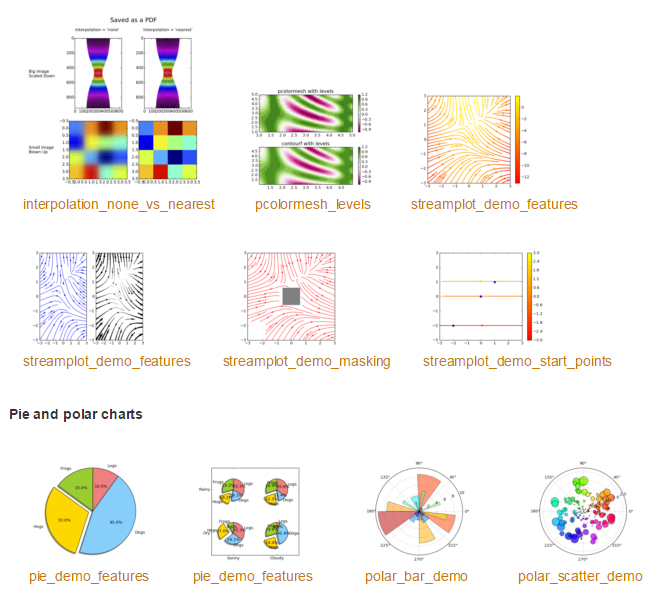
\includegraphics[height=0.8\textheight]{fig/matplotlibgallery}
	
\end{onlyenv}
\end{frame}
%%%%%%%%%%%%%%%%%%%%%%%%%%%%%%%%%%%%%%%%%%%%%%%%%%%%%%%%%%%%%%%%%%%%%%%%%%%%%%%%%
\begin{frame}[fragile]
	\frametitle{Bestanden inlezen}
	\begin{itemize}
		\item ascii: via file handler "\lstinline{with open('file.txt','r') as f:}"
		\item Volledige file in één keer als string "\lstinline{data = f.read()}"
		\item Lijn per lijn "\lstinline{for line in f:}"
		\item "\lstinline{\t}", "\lstinline{\n}"
		\item Speciale packages voor speciale formaten (\lstinline{csv}, \lstinline{openpyxl},...)
	\end{itemize}
	
	\lstinputlisting{examples/csvreader.py}
	
\end{frame}  	
%%%%%%%%%%%%%%%%%%%%%%%%%%%%%%%%%%%%%%%%%%%%%%%%%%%%%%%%%%%%%%%%%%%%%%%%%%%%%%%%%
\begin{frame}[fragile]
	\frametitle{Een project structureren}
\begin{onlyenv}<1>
	\begin{itemize}
		\item Gebruik functies
		\item Maak binnen functies gebruik van sub-functies indien nuttig
		\item Geef functies een betekenisvolle naam
		\item Groepeer functies die bij elkaar horen in een map en voeg deze map toe aan het Matlab pad
		\item Don't Repeat Yourself (DRY)
		\item Gebruik betekenisvolle namen voor variabelen
		\item Documenteer alles
	\end{itemize}
\end{onlyenv}
\begin{onlyenv}<2>
Voorbeeld folderstructuur:

	\begin{lstlisting}[language=bash]
mijnProject	
|-- data
|   |-- mijndata.csv
|
|-- lib
|   |-- __init__.py
|   |
|   |-- data
|   |   |-- __init__.py
|   |   |-- data_inlezen.py
|   |   |-- data_naar_coordinaten.py
|   |
|   |-- plot
|       |-- __init__.py
|       |-- plot_coordinaten.m
|
|-- main.py
|-- readme
	\end{lstlisting}
\end{onlyenv}
\begin{onlyenv}<3>

Voorbeeld main.py:
	\begin{lstlisting}
# main.py
# dit script leest data in, vertaalt deze in coordinaten
# en maakt een plot

# functies importeren
import lib

# data inlezen en bewerken
data = lib.data.data_inlezen('data/mijndata.csv')
[x,y,z] = lib.data.data_naar_coordinaten(data)

# plotten
lib.plot.plot_coordinaten(x,y,z)
	\end{lstlisting}	
	
\end{onlyenv}
\end{frame}
%%%%%%%%%%%%%%%%%%%%%%%%%%%%%%%%%%%%%%%%%%%%%%%%%%%%%%%%%%%%%%%%%%%%%%%%%%%%%%%%%
\begin{frame}
	\footnotesize
	\vspace{4cm}
	
\includegraphics[height=0.3cm]{fig/cc} \
	
\includegraphics[height=0.3cm]{fig/by} \
	
\includegraphics[height=0.3cm]{fig/sa}
	\quad \the\year\ Brecht Baeten
	\vspace{0.5cm}
	
    Dit werk is gelicenseerd onder de licentie Creative Commons Naamsvermelding-GelijkDelen 4.0 Internationaal. Ga naar http://creativecommons.org/licenses/by-sa/4.0/ om een kopie van de licentie te kunnen lezen.
    	
    \vspace{0.5cm}
    De bron van dit document en alle tekeningen zijn beschikbaar op https://github.com/BrechtBa/inleiding-tot-matlab
\end{frame}
%%%%%%%%%%%%%%%%%%%%%%%%%%%%%%%%%%%%%%%%%%%%%%%%%%%%%%%%%%%%%%%%%%%%%%%%%%%%%%%%%	
\end{document}